% !TeX spellcheck = en_GB
\begin{frame}{Implementation}
	\begin{itemize}
		\item<2->
		load CSV with Python

		\item<3->
		\emphblue{2D array} for the \emphblack{one-hot encoding} of the odour
		
		\item<4->
		Python package \emphblue{dgim} for the \emphblack{algorithm}
		
		\item<5->
		\emphblue{Streamlit} for the \emphblack{interface}
		
		\item<6->
		options
		\begin{itemize}
			\item<7->
			odour type
			
			\item<8->
			window size $N$
			
			\item<9->
			error rate
		\end{itemize}
	\end{itemize}

	\begin{picture}(0,0)(-215,-5)
		\includegraphics<5->[height=4cm]{images/overview.png}
	\end{picture}
\end{frame}

%\begin{frame}{}
%	\begin{figure}
%		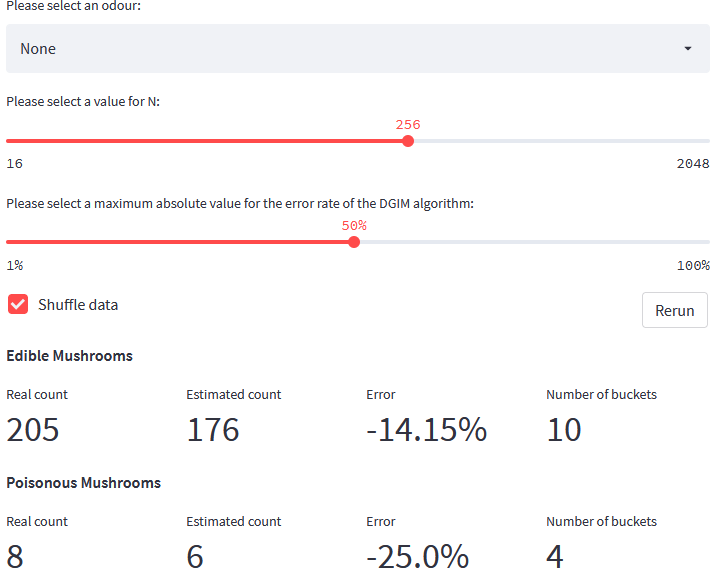
\includegraphics[height=.75\linewidth]{images/typical1.png}
%	\end{figure}
%\end{frame}

\begin{frame}{}
	\begin{figure}
		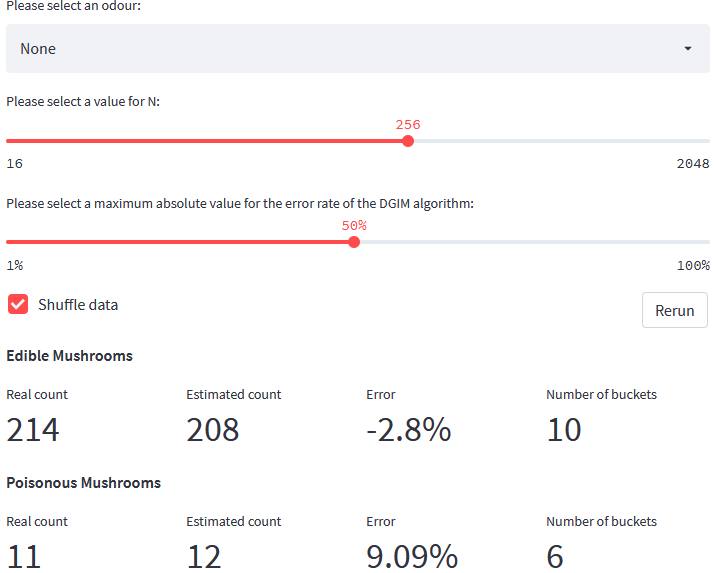
\includegraphics[height=.75\linewidth]{images/typical2.png}
	\end{figure}
\end{frame}

\begin{frame}{}
	\begin{figure}
		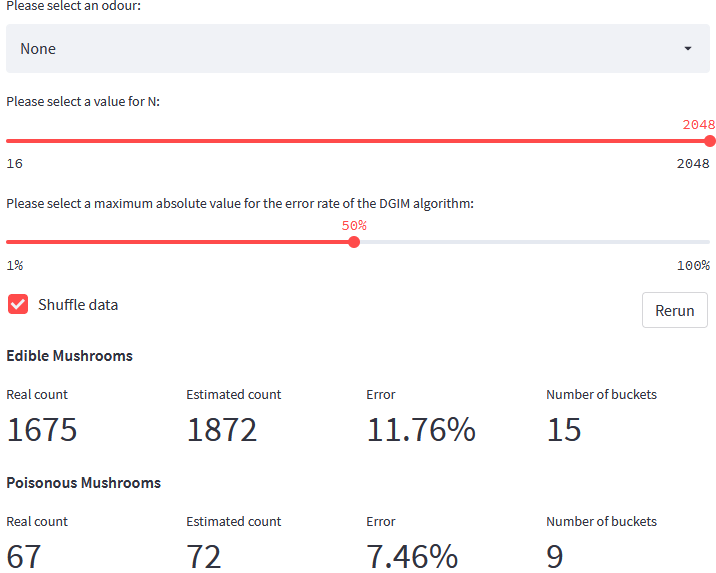
\includegraphics[height=.75\linewidth]{images/big_n.png}
	\end{figure}
\end{frame}

%\begin{frame}{}
%	\begin{figure}
%		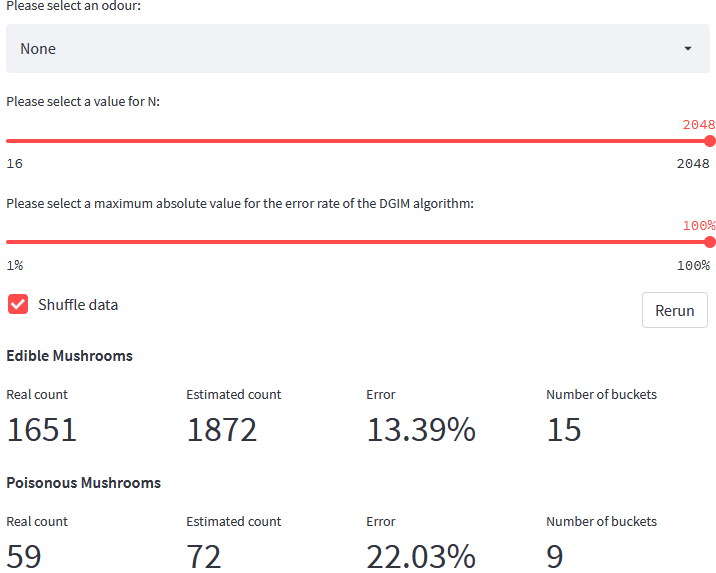
\includegraphics[height=.75\linewidth]{images/big_e.png}
%	\end{figure}
%\end{frame}

\begin{frame}{}
	\begin{figure}
		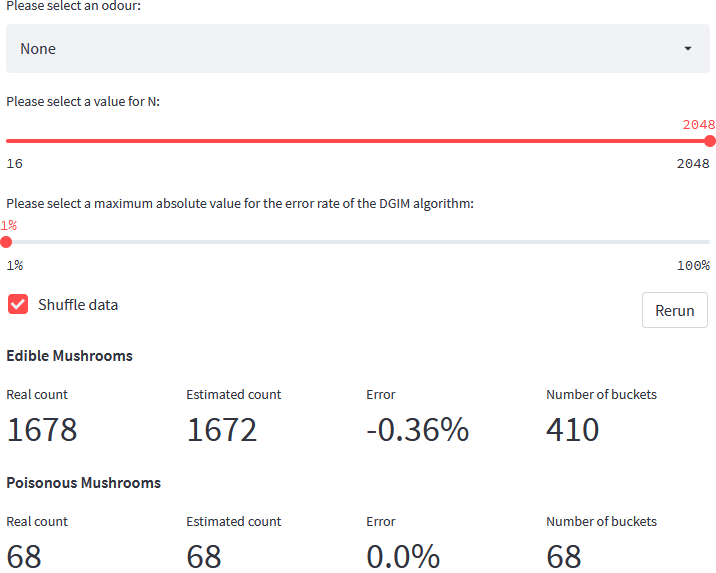
\includegraphics[height=.75\linewidth]{images/small_e.png}
	\end{figure}
\end{frame}